\section{INTRODUCTION}
%%% Motivation
%%%
In many data science and machine learning
tasks, the optimization of a discrete function
is required. For example, \textit{subset selection}
problems \citep{Wei2015,Kim2020}, 
such as selecting the most informative features from a dataset for model training.
As another example, consider the problem of selecting a subset of items to display
in a recommendation system \citep{Mehrotra2023,Ko2022}, where the goal is to maximize user engagement.

In this work, we consider maximization of an
objective function $f$ defined on subsets
of $\uni$, subject to a
knapsack constraint: a modular
cost function $c$ on the elements
is restricted to be at most the budget $\kappa$.
Denote by
$f_{\kappa}(X) = \max_{S \subseteq X : c(S)\le \kappa } f(S),$
where $X \subseteq \uni$. 
For many applications of this problem, the ground
set $\uni$ is massive, with size $n$ in the billion-scale
or larger. On the other hand, the budget constraints
are frequently such that an optimal set has only a few elements.
For example,
in viral marketing campaigns \citep{Kempe2003a},
a company may have a budget to promote
only a limited number of products while still aiming to
maximize overall sales or customer reach.
Intuitively, in these cases, the vast majority of elements of $\uni$ are irrelevant
to finding $f_{\kappa}(\uni)$.

Therefore, rather than solving $f_{\kappa}(\uni)$ directly,
it may be beneficial to produce a small set $\uni' \subseteq \uni$
of relatively promising candidate elements. Once $\uni'$
is obtained, an expensive
heuristic or exact algorithm may be employed to produce a feasible
solution.
Further, since elements not in $\uni'$ are discarded,
we desire a range of budgets $[\kappa_{\min}, \kappa_{\max}]$
to be supported, so that the pruned
ground set has value beyond a single use.
%We formulate the pruning problem formally in Section
%\ref{sec:prelim}. 
Formally, we have the following problem definition.

\textbf{Problem definition (Pruning).}
Given an objective function $f: 2^\uni \to \mathbb{R}_+$,
modular cost function $c: \uni \to \mathbb{R}_+$,
and budget range $[\kappa_{\min}, \kappa_{\max}]$,
produce $\uni' \subseteq \uni$,
such that
\begin{itemize}
\item $|\uni'| = \oh{ F( \kappa_{\max}, \kappa_{\min}, c ) \polylog(n)},$ where $F$ is a function and $n = |\uni |$; 
\item there exists $\alpha \in [0,1]$, such that, for any $\tau \in [\kappa_{\min}, \kappa_{\max}]$,
  it holds that $f_{\tau}( \uni' ) \ge \alpha f_{\tau }( \uni ).$
\end{itemize}

Existing methods for the pruning task \citep{Zhou2017,Manchanda2020a,Ireland2022,Tian2024} are heuristics
that 1) are only formulated to solve one instance of size-constrained maximization;
2) provide no guarantee on the size of $\uni'$; and
3) provide no guarantee on the fraction of the optimal value retained in $\uni'$ after the pruning process. Thus, in this work, we are motivated by the following
questions:
\begin{center}
  \textit{Is it possible to develop pruning algorithms with theoretical guarantees that are useful beyond solving one problem instance?
    If so, what assumptions are required on the objective function and the problem instance?
    Are the resulting algorithms practical and competitive with existing heuristics?}
\end{center}


\begin{figure*}[t] 
  \centering
  \subfigure[] {
    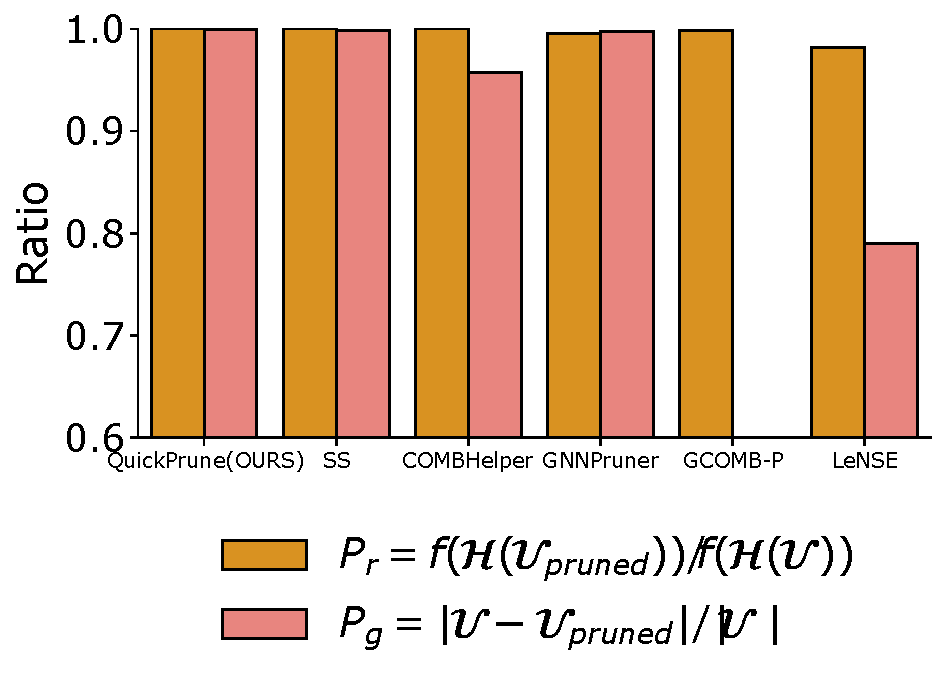
\includegraphics[width=0.45\textwidth]{Figures/MaxCover_performance_inkspace.pdf}
  }
  \subfigure[] {
    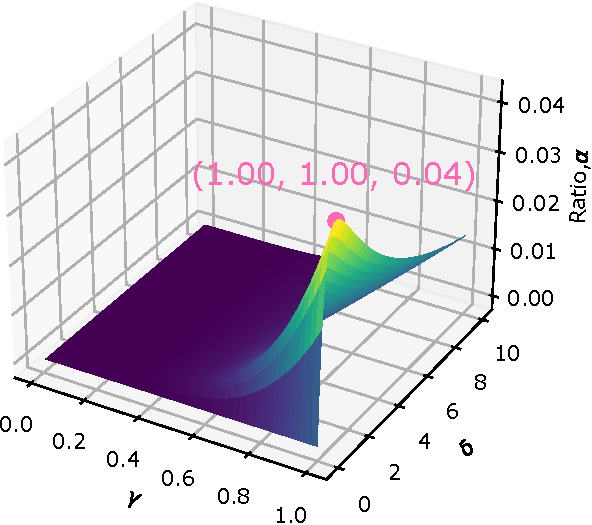
\includegraphics[width=0.45\textwidth]{Figures/3d_plot_max_label_crop_inkspace.pdf}
  }
  
  \caption{\textbf{(a):} Typical empirical results of \qs versus competing methods on an instance of the MaximumCover problem: \qs retains
    99.99\% of the optimal value while pruning $99.95\%$ of the ground set.
  \textbf{(b):} Plot of the pruning ratio $\alpha (\epsi, \delta, \gamma )$ of Theorem \ref{thm:multi}, as a function of the parameter $\delta$ of \qs and the $\gamma$-submodularity of the objective function $f$. Here, $\epsi$ is fixed to $0.01$.} 
  \label{fig:intro-fig}
\end{figure*}

\textbf{Contributions.} 
 We introduce \qs{}, a lightweight pruning method that
 prunes the original ground set $\uni$
 for a range of budgets in a single pass
 through the ground set.
 We emphasize that lightweight pruning methods
 are needed since an expensive pruning process defeats the
 purpose of pruning. In this regard, our algorithm
 processes elements one-by-one -- once an element is rejected,
 it is never re-considered and may be safely discarded.
 \qs{}  makes at most $\oh{\log ( \kappa_{\max} / \kappa_{\min} )}$
 queries to $f$ per element processed. 
 Moreover, we prove theoretical bounds
 on the quality of the pruned ground set $\uni'$ of \qs{}, and also
 on its size.

 Specifically, given budget range $\kappa_{\text{min}} \le \kappa_{\text{max}}$, we show that
 the output of \qs{} satisfies
$| \uni' | = \oh{ \log \left( \frac{ \kappa_{\max} }{ \kappa_{\min} } \right) \cdot \left( \frac{\kappa_{\max}}{ c_{\min}} \right) \log ( n)}$, where $c_{\min} = \min_{u \in \uni} c(u)$. 
Further, if the objective function $f$ is $\gamma$-weakly
submodular\footnote{Submodularity is a diminishing-returns condition ubiquitous to many applications, discussed further in Section \ref{sec:prelim}.}, and if a mild assumption\footnote{Namely, that no single element uses almost all of the budget. See Section \ref{sec:alg} for the precise formulation.} on the costs of elements in
 an optimal solution of $f_{\tau}(\uni )$ holds, we show
 that
 $f_{\tau} ( \uni' ) \ge \alpha( \epsi, \delta, \gamma ) \cdot f_{\tau} ( \uni )$,
 for any $\tau \in [\kappa_{\min}, \kappa_{\max} ]$, where $\epsi, \delta$
 are parameters of the algorithm. A plot of $\alpha$ is shown in Fig. \ref{fig:intro-fig}(b);
 If $\gamma = 1$ and $\delta = 1$,
 $f_{\tau} ( \uni' ) \ge \left( \frac{1}{24} - \epsilon \right) f_{\tau} ( \uni )$.
 To the best of our knowledge, all previous methods for this
 problem are heuristics with no performance guarantee, either on
 the size of the pruned universe or on the fraction of the optimal
 value retained after pruning. We give a comprehensive discussion
 of related work in Section \ref{sec:related-work}. 

 % Moreover, our method
 % handles general knapsack constraints, while
 % most previous methods were designed for size constraint only, and
 % it is unclear how they could be generalized to more sophisticated
 % constraints without substantial changes, as discussed in
 % Section \ref{sec:related-work}. 
 
 To show the practical effectiveness of our algorithm,
 we evaluate it against several
 state-of-the-art classical and machine learning heuristics
 for the pruning problem across four different optimization contexts.
 The methods are evaluated by two metrics, the fraction $P_g$ of the
 original ground set that is pruned (higher is better); and the fraction $P_r$ of the
 value of a solution by a given algorithm $\mathcal H$ for the problem
 that is retained (higher is better);
 \ie $P_r = f( \mathcal H ( \uni' ) ) / f( \mathcal H ( \uni ) )$.
 Empirically, as shown in Fig. \ref{fig:intro-fig},
 our algorithm outperforms competing methods on both metrics,
 and achieves substantial reductions in
 ground set size (typically over 90\%) while nearly preserving the
 value of $f_\kappa $ across multiple budgets.

 \textbf{Organization.} The rest of this paper
 is organized as follows. In Section \ref{sec:related-work},
 we describe the relationship of our contribution to existing
 work; in Section \ref{sec:prelim}, we introduce preliminaries
 and notation. In Section \ref{sec:alg}, we describe our
 \qs algorithm and prove Theorem \ref{thm:multi}, which
 summarizes its theoretical properties. In Section \ref{sec:exp},
 we conduct our empirical evaluation and comparison to existing
 heuristics for the pruning problem. In Section \ref{sec:con},
 we conclude the paper and discuss future directions.
 In Appendices, we describe omitted details and proofs from the main text.

\subsection{Related Work} \label{sec:related-work}
\textbf{(Weakly) Submodular Optimization.}
\textit{Submodularity} is a notion of diminishing
returns that is satisfied or partially satisfied
by many, varied objective functions \citep{Demeniconi2021, Feige, Feige1996, Feige2011, Feige2011a, Feige2013, Gharan2010, Gharan2011, Gharan2011a, Gharan2011b, Gupta2010a, Khot2001, Kothawade2022, Lee2009, Nemhauser1978b, Uziahu2023, Vondrak2013}.
Constrained non-submodular maximization has proven useful for
data summarization (\eg \citep{Demeniconi2021,Kothawade2022}), feature selection \citep{Elenberg2018},
reduction of training set size 
for deep learning methods \citep{Killamsetty2023}.
Submodularity occupies a role for discrete optimization
analagous to the role of convexity in continuous optimization.
% Therefore, the class of optimization problems we
% consider are of the form $\max_{S \in \isets} f(S)$,
% where $\isets$ are the set of feasible subsets of the ground
% set, and $f$ is a partially submodular, partially monotone
% objective function. Thus, as elaborated below, we seek to
% find small sets $\uni' \subseteq \uni$, such that $\max_{S \cap \uni' : S \in \isets} f(S \cap \uni')$ is degraded by
% only a small, bounded amount over the original problem.
The typical model (\eg \citep{Feige, Gharan2011a, Gupta2010a}) is that the function $f$ is
available to an algorithm as a black-box orcale
that returns $f(S)$ when queried with set $S$. However,
these function evaluations are very expensive, so we
desire to minimize the \textit{query complexity} of an algorithm. 

\textbf{Coresets.}
Our notion of pruning is related to the
idea of a coreset \citep{Braverman2022, Feldman2020b, Indyk2014, Kogan2015, Liu2019, Mirrokni2015, Mirzasoleiman2020, Tukan2020, Tukan2022, Yang2023a, Zhang2022e}; in which
a small set is to be selected to
best summarize a set of
points with respect to a desired
set of queries; for example,
construct a weighted graph that
approximately preserves the values
of every cut in an original graph
\citep{Kogan2015}. 
The concept of coreset does not
have a precise definition,
and thus our 
terminology
\textit{pruned universe}
could be
recast as coreset. 
Coresets have been applied
to \eg graph summarization \citep{Liu2019},
data-efficient training of ML models \citep{Mirzasoleiman2020,Yang2023a},
pruning neurons from neural networks \citep{Tukan2022}.
For the types of optimization
problem we consider, \ie
constrained maximization with objective
function available as a value query oracle,
there have been only a small
number of attempts to produce a coreset
\citep{Indyk2014,Mirrokni2015}.
The closest to our setting
is the method of \citet{Mirrokni2015}.
Their notion of \textit{randomized
  composable coreset}
is used for distributed computation
and is only applicable to
a single size constraint. 
Also, their notion of coreset
is much stronger than what we require
in this work. 
% (and sufficient conditions and proposed generalizations thereof)
% will be useful in combination with
% our proposed pruning algorithms,
% especially for the distributed setting, as we
% elaborate below. 

\textbf{Pruning via supervised learning methods.}
There have been multiple ML-based heuristics
proposed to accomplish the pruning task
for a single instance of a combinatorial optimization
problem.
The first line of work \citep{Lauri2019, Lauri2023, Sun2021b, Sun2021c, Zhang2022b}
seeks to train a binary classification algorithm to predict
whether a data element belongs to an optimal solution.
These approaches
consider graph-based optimization problems and
train a linear classifer on vertices
by hand-crafting a set of local features for each vertex,
such as centrality measures,
solutions to linear programming relaxations, and so on; a classifier, such as random forests, is then trained on small instances that can be exactly solved. The goal is to correctly predict when a vertex does \textit{not} belong to an optimal solution,
and hence can be safely pruned. 
These methods rely on hand-crafted features
customized to each problem; which themselves may
be superlinear to compute, such as a
solution to an LP relaxation of the problem
or the eigenvector centrality on the original (unpruned)
graph.
A recent generalization (COMBHelper) of this approach uses a GCN (graph convolution network)
in place of a linear classifer \citep{Tian2024}.
We compare to COMBHelper empirically in Section \ref{sec:exp}. 

\textbf{Other heuristics for pruning.}
GCOMB \citep{Manchanda2020a}
uses a weighted degree heuristic
with a probabilistic greedy algorithm,
combined with a supervised learning approach, to produce a pruned
ground set. On the other hand, LeNSE \citep{Ireland2022} trains an RL agent to navigate from an initial subgraph to a pruned subgraph that most likely contains the optimal solution for a specific optimization problem via a local search procedure on subgraphs.
Another heuristic is that of \citet{Zhou2017}, which uses ideas from submodularity
to extract a promising pruned universe. We empirically compare our algorithm
to each of these methods in Section \ref{sec:exp}. In contrast to our work,
all of these are formulated
for a single instance of size-constrained maximization and have no theoretical
guarantees of any kind, \textit{including that a nonempty feasible solution remains after the
pruning process}. 

% In recent years, several classical and machine learning-based methods have been developed to reduce the search space in combinatorial optimization (CO) problems. \cite{zhou2017scaling} proposed Submodular Sparsification, a randomized pruning method using a submodularity graph, outperforming Lazy Greedy \citep{minoux2005accelerated} and Sieve-Streaming \citep{badanidiyuru2014streaming}. \cite{manchanda2020gcomb} proposed GCOMB, a combination of hand-crafted heuristic and graph neural network (GNN), to prune nodes unlikely to be part of the solution set for the Maximum Coverage and Influence Maximization. \cite{lauri2019fine} proposed a probabilistic preprocessing framework using a classifier based on graph-theoretic and statistical features for the Maximum Clique Enumeration problem. This was extended by \cite{grassia2019learning} with a multi-stage classifier that further prunes the search space, achieving substantial speedups. Instead of pruning vertices, \cite{ireland2022lense} introduced a GNN-based local search method to extract subgraphs. Most recently, \cite{tian2024combhelper} introduced COMBHelper, leveraging GNNs with knowledge distillation and weight boosting to improve vertex classification.

\subsection{Preliminaries and Notation} \label{sec:prelim}
For natural number $n$, we use the notation $[n] = \{0, 1, \ldots, n-1 \}$,
and for a function $f$ understood from context: $\marge{T}{S} = f( S \cup T ) - f(S)$
is the \textit{marginal gain} of set $T$ to set $S$. 
A non-negative set function on ground set $\uni$, $f : 2^\uni \to \mathbb R^+$,
is \textit{submodular} iff
$\forall S \subseteq \uni, \forall T \subseteq \uni, f( S \cap T ) + f( S \cup T ) \le f(S) + f(T).$
Roughly speaking, this means the whole is not greater than the sum of its parts.
An equivalent characterization is the following notion of diminishing-returns:
$ \forall S \subseteq T \subseteq \uni, \forall x \not \in T, \marge{x}{T} \le \marge{x}{S}.$
A non-negative, set function $f$ 
is \textit{monotone} iff
$\forall S \subseteq T \subseteq \uni, f( S ) \le f( T ).$
A submodular function is not necessarily monotone.

In this work, we consider the following relaxation of
submodularity: the monotone function $f$ is $\gamma$-submodular
iff $\gamma$ is the maximum
value in $[0,1]$ such that $\forall S \subseteq T \subseteq \uni, \forall x \not \in T, \gamma \marge{x}{T} \le \marge{x}{S}.$
Observe that $f$ is submodular iff $\gamma = 1$. 
Occasionally in the literature, $\gamma$ is termed the \textit{diminishing-returns ratio} of a function
\cite{Bian2017b,Kuhnle2018}.
We remark that monotonicity is needed for the definition of $\gamma$-submodular,
and throughout our analysis, we assume that the objective function $f$ is monotone. 

%%% Local Variables:
%%% mode: latex
%%% TeX-master: "main.tex"
%%% End:
